\documentclass[letterpaper, 12pt]{math}

\usepackage{graphicx}

\geometry{letterpaper, margin=0.5in}

\title{Intro to Computer Science Theory: Homework 3}
\author{Alvin Lin and Joshua Cotton}
\date{August 2017 - December 2017}

\begin{document}

\maketitle

\subsection*{Problem 1}

\begin{enumerate}
  \item Consider the following languages, each defined over the alphabet
  \( \{a,b\} \)
  \begin{enumerate}
    \item \( L_1 = \{x\mid|x|\geq3\text{ AND its third symbol from the right
    is } b\} \)
    \item \( L_2 = \{x\mid x\text{ contains at least two } b\text{s OR at most
    one } a\} \)
    \item \( L_3=\{x\mid\text{starts with }a\text{ AND has even length, OR
    starts with } b \text{ AND has odd length}\} \)
  \end{enumerate}
  Each of these languages is ``complex,'' in the sense that it can be broken
  into the union or intersection of simpler languages, where each simpler
  language is defined by one of the clauses of the set builder between ``OR''
  or ``AND.'' For instance, the first set can be redefined as
  \[ L_1 = \{x\mid|x|\geq 3\} \cap \{x~|~x\mbox{'s third symbol from the right
    is } b\} \]
  \begin{enumerate}
    \item ~[2 points each] For \( L_2 \) and \( L_3 \) above, rewrite each of
    the definitions by removing all AND's and OR's and replacing them with the
    intersection or union of simpler sets based on each clause (as in the
    example for \( L_1 \) given above). Note that for \( L_3 \) this means you
    need four simple sets and parentheses to make your definition clear.
    \[ L_2 = \{x\mid x\text{ contains at least two } b\text{s}\} \cup \{x\mid
      x\text{ contains at most one } a\} \]
    \begin{align*}
      L_3 =& \bigg(\{x\mid x\text{ starts with } a\}\cap\{x\mid x\text{ has even
        length}\}\bigg)\cup\ \\
      & \bigg(\{x\mid x\text{ starts with } b\}\cap
        \{x\mid x\text{ has odd length}\}\bigg)
    \end{align*}
    \item ~[1 point for each simple language, 8 points total] For each of the
    simple sets (two simple sets for \( L_1 \) and \( L_2 \), four for
    \( L_3 \)), provide the state transition diagram for each. Label the states
    for each machine.
    \[ \{x\mid x\text{ contains at least two } b\text{s}\} \]
    \begin{center}
      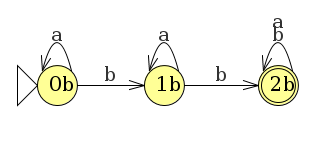
\includegraphics[width=8cm]{hw_3_1.png}
    \end{center}
    \[ \{x\mid x\text{ contains at most one } a\} \]
    \begin{center}
      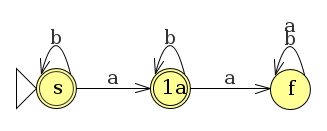
\includegraphics[width=8cm]{hw_3_2.png}
    \end{center}
    \[ \{x\mid x\text{ starts with } a\} \]
    \begin{center}
      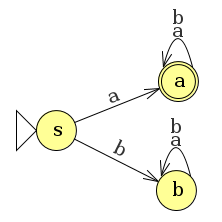
\includegraphics[width=5cm]{hw_3_3.png}
    \end{center}
    \[ \{x\mid x\text{ has even length}\} \]
    \begin{center}
      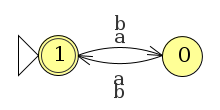
\includegraphics[width=5cm]{hw_3_4.png}
    \end{center}
    \[ \{x\mid x\text{ starts with } b\} \]
    \begin{center}
      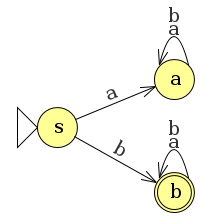
\includegraphics[width=5cm]{hw_3_5.png}
    \end{center}
    \[ \{x\mid x\text{ has odd length}\} \]
    \begin{center}
      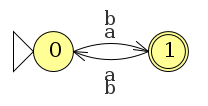
\includegraphics[width=5cm]{hw_3_6.png}
    \end{center}
    \[ \{x\mid|x|\geq3\} \]
    \begin{center}
      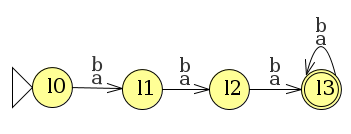
\includegraphics[width=8cm]{hw_3_7.png}
    \end{center}
    \[ \{x\mid x\text{'s third symbol from the right is } b\} \]
    \begin{center}
      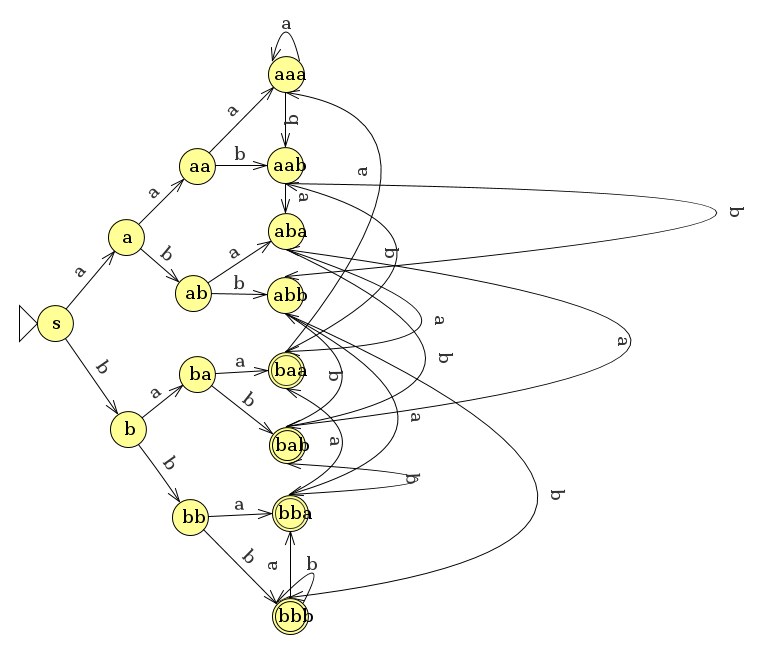
\includegraphics[width=12cm]{hw_3_8.png}
    \end{center}
    \item~[4 points for each complex language, 12 points total] For each of the
    three complex languages \( L_1 \), \( L_2 \), and \( L_3 \), use the
    construction from Theorem 1.25 (and the discussion in the footnote below)
    to construct FAs for each from the simple sets. You need only draw the
    state transition diagrams for each complex language, but the state names,
    accepting states etc. must reflect the construction. Note also that for
    \( L_1 \) and \( L_2 \) you need apply the construction once, but for\
    \( L_3 \) you need to apply it three times.
    \[ L_1 \]
    For \( L_1 \) the language \( \{x\mid|x|\geq3\} \) is a subset of the
    language \( \{x\mid x\text{'s third symbol from the right is } b\} \), thus
    the state transition diagram for \( \{x\mid x\text{'s third symbol from the
    right is } b\} \) is also the state transition diagram for \( L_1 \).
    \begin{center}
      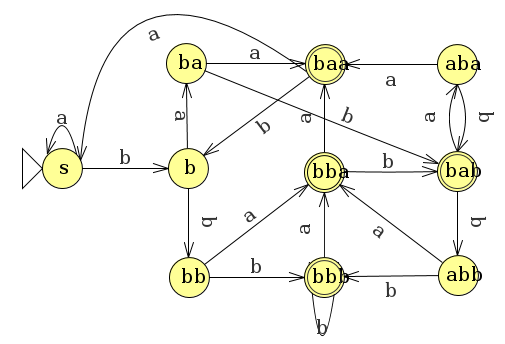
\includegraphics[width=8cm]{hw_3_l1.png}
    \end{center}
    \[ L_2 \]
    \begin{center}
      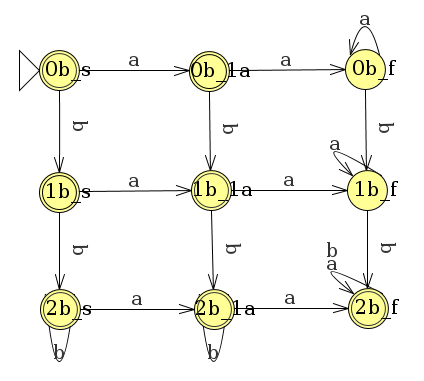
\includegraphics[width=8cm]{hw_3_l2.png}
    \end{center}
    \[ L_3 \]
    \begin{center}
      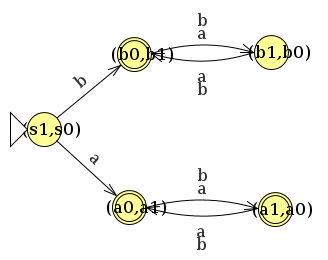
\includegraphics[width=8cm]{hw_3_l3.png}
    \end{center}
  \end{enumerate}
  \item For any alphabet \( \Sigma \), consider the following (recursive)
  definition of \( |\cdot|: \Sigma^* \rightarrow \mathbb{N}\) (where
  \( \mathbb{N} \) is the natural numbers, PLUS \( 0 \)), on input \(x \in
  \Sigma^*\) and \(y \in \Sigma\) as
  \[ |x| = \left\{\begin{array}{ll} 0 & \mbox{ if } x = \epsilon \\
    |y| + 1 & \mbox{otherwise, where } x=ya \wedge y \in \Sigma^* \wedge a \in
    \Sigma.\end{array}\right. \]
  \begin{enumerate}
    \item ~[3 points] Write the following statement in quantifiable logic:
    ``For any alphabet \( \Sigma \), \( z,w\in\Sigma^* \), and \( b\in\Sigma
      \), if \( |zw| = |z| + |w| \) then \( |zwb| = |z| + |w| + 1 \).''
    \[ \forall{\Sigma}\bigg(\forall{z}\forall{w}\forall{b}(z,w\in\Sigma^*\wedge
      b\in\Sigma\wedge|zw| = |z|+|w| \to |zwb| = |z|+|w|+1)\bigg) \]
    \item ~[3 points] Finish the proof. For each quantifier, you must use one
    of the proof strategies from Velleman. Use square brackets and logical
    forms to cite each use of a strategy, as in page 27--28 of the course notes.
    \begin{enumerate}
      \item ~[The statement is of the form \( \forall{x}P(x) \)]
      Let \( \Sigma \) be an arbitrary alphabet.
      \item ~[The statement is of the form \( \forall{b}P(b) \)]
      Choose an arbitrary \( b \).
      \item ~[The statement is of the form \( R\to S \)]
      Suppose that \( \forall{z}\forall{w}(z,w\in\Sigma^*\wedge
      b\in\Sigma\wedge|zw| = |z|+|w| \), we need to show that \( |zwb| =
      |z|+|w|+1 \).
      \item By the definition \( |x| = |y|+1 \text{ where } x=ya\wedge y\in
      \Sigma^*\wedge a\in\Sigma\), it follows that \( |zwb| = |zw| + 1 \).
      \item From what is given, \( \forall{z}\forall{w}|zw| = |z|+|w| \), it
      follows that \( |zwb| = |z|+|w|+1 \)
    \end{enumerate}
  \end{enumerate}
\end{enumerate}

\begin{center}
  If you have any questions, comments, or concerns, please contact me at
  alvin@omgimanerd.tech
\end{center}

\end{document}
